\section{Evaluation}

We conducted a user study to evaluate Narvis, 
comparing the authoring experience and output generated by Narvis and a general presentation tool, i.e., PowerPoint.
% and gained insights on how the authoring experience and output would compare to slideshows created with general presentation tools. 
Our study was a between-subjects design with two sample groups: one group of participants used Narvis, the other group used PowerPoint
% , which is widely used to create presentation slideshow. 
We report our qualitative observations during the authoring process, and provide insights on the quality of the slideshows generated from both groups.

\subsection{Participants}
We invited 4 experts in data visualization to this user study as editor participants, denoted as PC1 and PC2 for the control group, PE1 and PE2 for the experiment group. All of them have more-than-one-year experience in the design and implementation of data visualization. We also sent emails to students in the data visualization course we mentioned before and recruited 20 volunteers to evaluate the quality of the generated slideshow as audiences, denoted as PAs. 
%\textbf{Audience }are novice in data visualization. They will review the slideshow produced by the experts, rate it, give subjective comments, and answer a series of questions to check their understanding of this visualization.\par
%For editors, we have 4 postgraduate students, aging between 22-30, and all of them have more than one year experience in data visualization.\par
%For audiences, we have 20 under graduate students, whose majors vary from business to biology. 
%According to the questionnaire, none of them have accessed advanced data visualization before. Only 13\% students know the tree map, and none can give a accurate explanation of theme river with topic splitting and merging.  \par
\subsection{Material}
We extracted the visual design and the corresponding literature description from  a visualization design paper ``TextFlow: Towards Better Understanding of Evolving Topics in Text''\cite{cui_textflow:_2011}.
We chose \textit{TextFlow} based following considerations. First, it's not too difficult for a novice but still a novel design that requires extra effect to clarify.
Second, it is a typical abstract data visualization that fully consists of graphical elements, which is in the coverage of our edge detection algorithm. 
Third, it visualizes evolving topics in social media, which is an interesting topic and can increase the engagement of audiences. 

This visualization design conveys multiple level results of topic evolution analysis: a set of topics
with splitting/merging relationships among each other, which encodes a series of topic flows, a set of critical events, which encodes glyphs, and the keyword correlations, which encode threads.  

\subsection{Procedure}
\subsubsection{Generating Slideshows}
We ran 90-min long sessions for the four participants separately. This session consisted of 3 phases: (1) \textit{Learning Phase}, (2) \textit{Sketch Phase}, (3) \textit{Authoring Phase}.

In the \textit{Learning Phase}, participants read the literature description we extracted from the paper, which offered a detailed description of the visual design with diagrams. This phase ended when the participants reported the experimenters that they finished reading and understand this visual design. 
This phase took 15 min, 14 min, 17 min and 13 min for 4 participants respectively.

In the \textit{Sketching Phase}, participants were asked to sketch ideas for introducing \textit{TextFlow}. They were encouraged to give considerations to (i) convey the insight to the people with less experience in data visualization; (ii) organize a clear narrative structure; (iii) think about additional annotation and animation required. Participants are asked to think aloud and experimenters are present in the room to observe. 

In the \textit{Authoring Phase}, participants implemented the ideas in their sketch as detailed as possible in a one-hour-long session to produce a narrative slideshow that can be self-explanatory. We send each participant a PNG file and a txt file as the raw material for authoring. Participants in control group use Power Point, a presentation making tool that all the participants are familiar with. In the experimental group, before authoring, experimenters demonstrate the working flow of Narvis through an automatic step by step tutorial included in Narvis. This training lasted about 15 min and is not counted in the one-hour authoring session. Participants are also allowed to ask additional questions in the authoring phase.

\subsubsection{Evaluation Methods}
The evaluation focus on two parts, the authoring experience of Narvis and the quality of the generated slideshows. We report our observation of the authoring experience based on an interview with the two PEs and the video we took during the authoring session. 
To evaluate the slideshows generated from both groups, we first analyzed the slideshows and reported some quantitative observations, such as the number of slides.
Then, to get an independent opinion, we asked 20 PAs to evaluate the generated slideshows. To eliminate the errors introduced by other variables such as the different watching environment, this part was conducted in a website we built. Each PA was randomly assigned a slideshow when visited this website. They watch all the slides by clicking two buttons, ``next'' and ``previous'', and their click activity was automatically recorded by a background program.  After watching the slideshow, they were asked to finish an online questionnaire composed of 2 parts: 1) a quiz about the visual design of ``TextFlow'' (with a full mark of 5);2) rate the slideshow  from 1 (very poor) to 5(excellent) at various aspects. 

\section{Results}
%We analyzed the following material: 1) video and notes that the experimenters took during the user study session, which the participants consented to. 2) the slides and the sketch created by participants, 3) the interview with the editor participants, 4) the ranking, comments, answers, click stream data from the audience participants. 

\subsection{Generated Slideshow}
We obtained 2 slideshows from the control group, denoted as SC1 and SC2, and 2 slideshows from the experiment group, denoted as SE1 and SE2(see in Figure~\ref{fig:user_study}). 


\begin{table}
  \caption{A summary of 4 slideshows}
  \label{tab:slides1}
  \small
  \centering
  \begin{tabu}{p{2cm}|p{0.9cm}|p{0.9cm}|p{0.9cm}|p{0.9cm}}
  \toprule
 \textbf{} &\textbf{SE1} & \textbf{SE2} & \textbf{SC1}& \textbf{SC2} \\ 
   \midrule
  \textbf{Number of Slides } & 29  & 22 & 7 & 3 \\ 
 \midrule
  \textbf{Average Reading Time(Total,s)} & 327.05 & 156.78 & 169.33 & 128.84\\ 
 \midrule
  \textbf{Averrage Reading Time(Per Slide, s)} & 11.27 & 7.09 &24 & 42\\ 
   \midrule
  \textbf{Information Missing (in Slideshow/in Sketch) }& 1/4 & 0/3 & 2/3 & 2/2\\ 
     \midrule
  \textbf{Average Length of Text (per Slide) }& 10.7 & 12.3 & 32 & 47\\ 
    
  \bottomrule

  \end{tabu}
  \vspace{1mm}
\end{table}



%\begin{table}[tb]
%  \caption{The questionnaire result}
%  \label{tab:slides2}
%  \small
%  \centering
%  \begin{tabular}{p{1.5cm}|p{0.9cm}|p{0.9cm}|p{0.9cm}|p{0.9cm}}
%  \toprule
% \textbf{} &\textbf{SE1} & \textbf{SE2} & \textbf{SC1}& \textbf{SC2} \\ 
%   \midrule
%  \textbf{Quiz Score } & 3.75  & 3.17 & 2.6 & 3.0 \\ 
% \midrule
% \midrule
%  \textbf{Readability} & 3.8 & 3.5 & 3.2& 2.75\\ 
% \midrule
%  \textbf{Utility} & 3.875 & 3.375 & 2.4 & 3.35\\ 
%   \midrule
%  \textbf{Aesthetics }  & 4.125 & 3.4 & 2.1& 2.75\\ 
%  \midrule
%  \textbf{Attractiveness} & 3.9 & 3.3 & 2.2 & 2.5\\ 
%  
%  \bottomrule
%
%  \end{tabular}
%  \vspace{1mm}
%\end{table}

\begin{figure}
 \centering % avoid the use of \begin{center}...\end{center} and use \centering instead (more compact)
 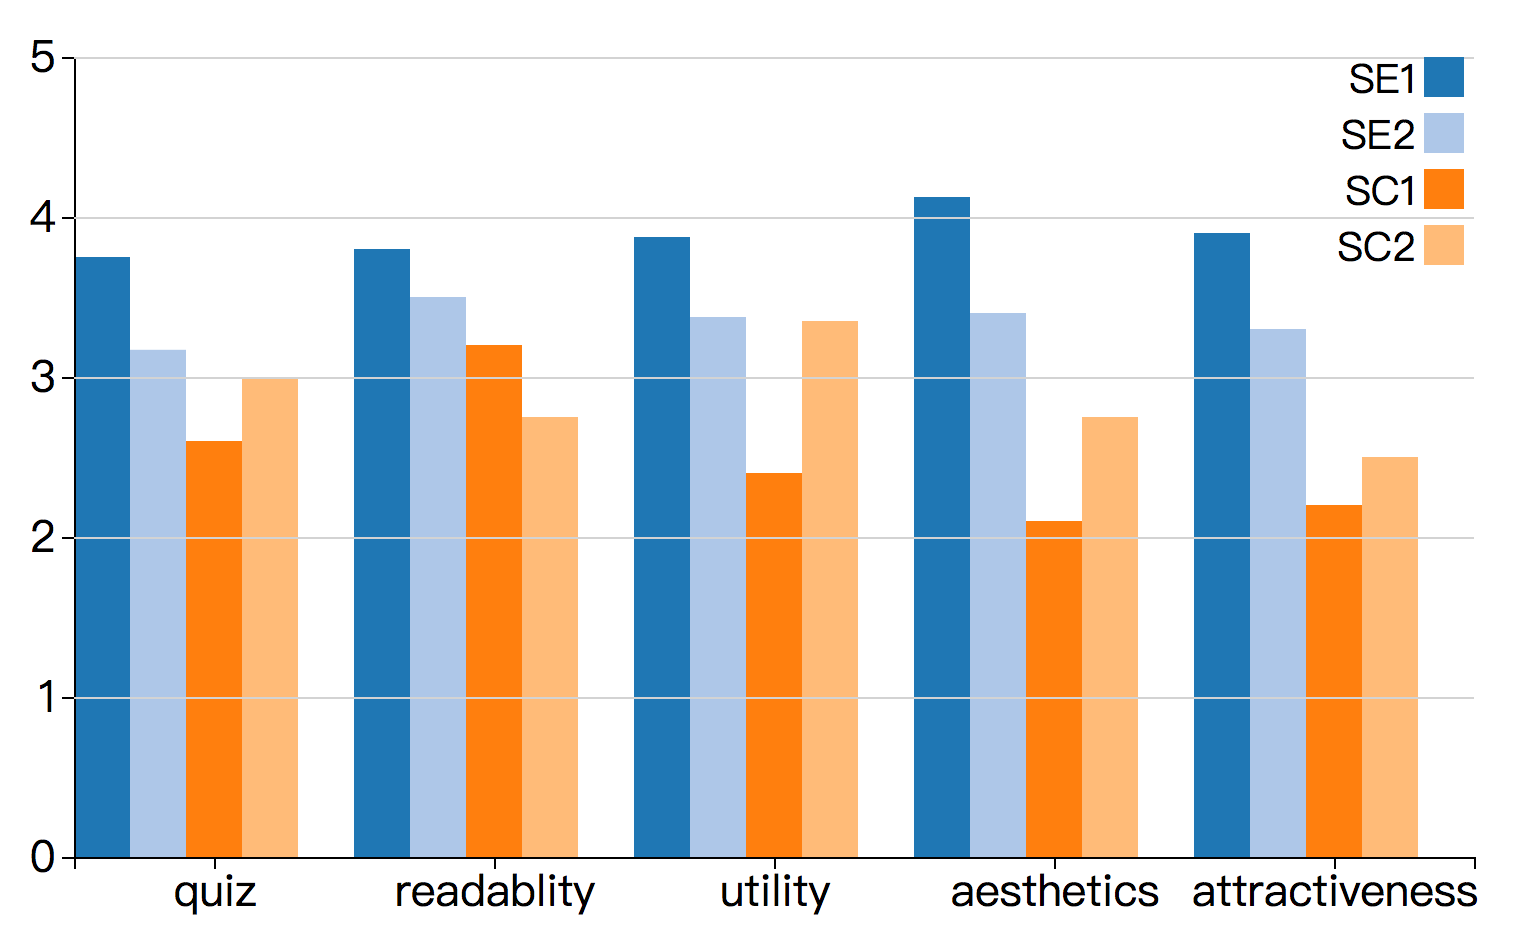
\includegraphics[width=\columnwidth]{questionnaire}
 \caption{The questionnaire results of 4 slideshows
 }
 \label{fig:questionnaire}
\end{figure}

\begin{figure}
 \centering % avoid the use of \begin{center}...\end{center} and use \centering instead (more compact)
 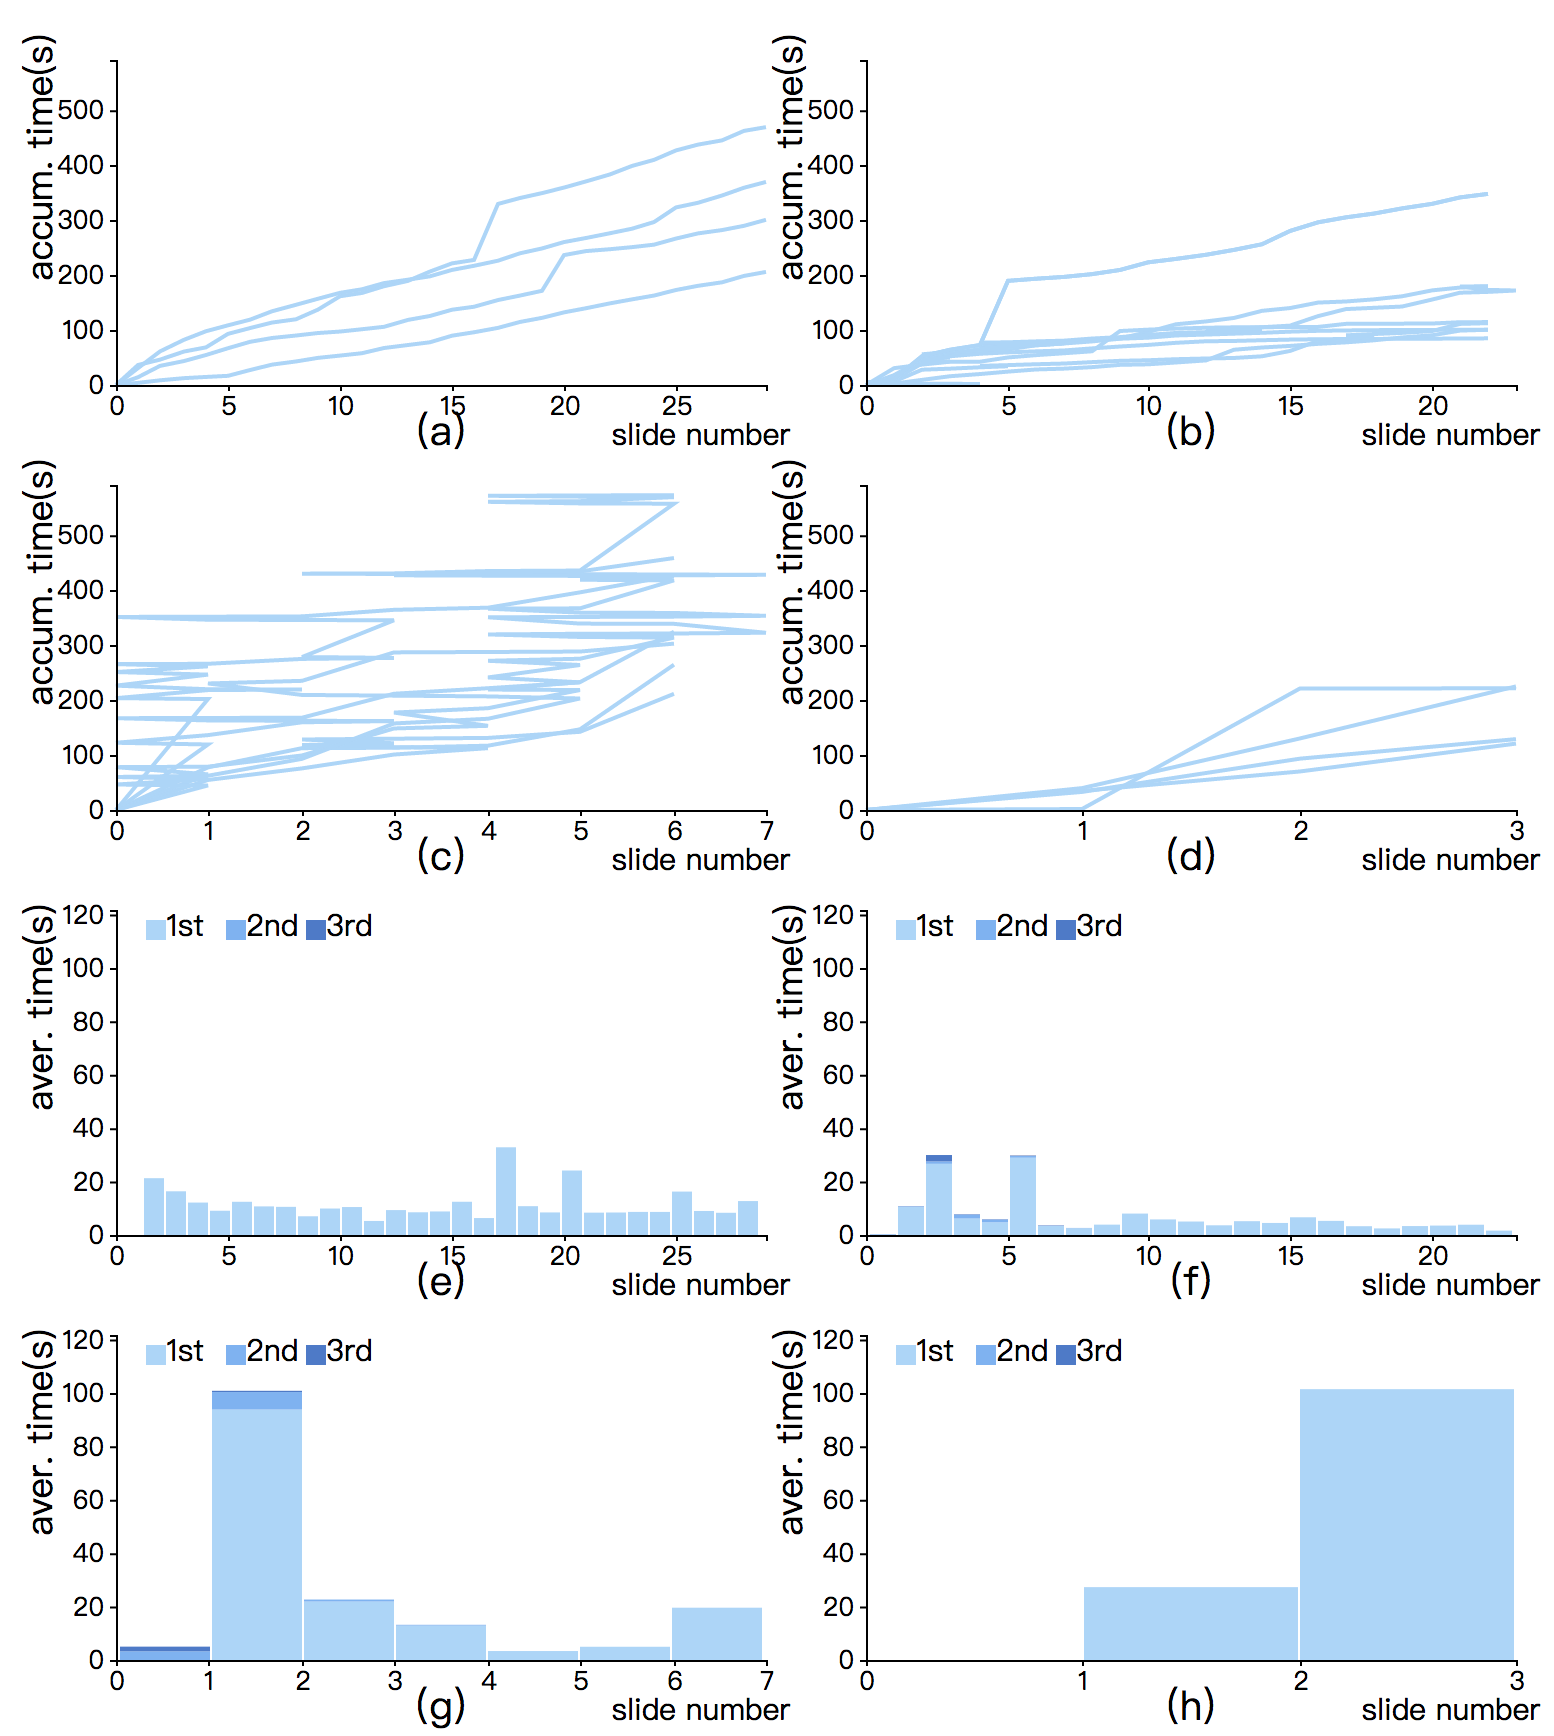
\includegraphics[width=\columnwidth]{clickstream}
 \caption{The visualization of clickstream data when PAs watch the slideshows created by PE1(a)(e), PE2(b)(f), PC1(c)(g), and PC2(d)(h), respectively. 
%The x axis represents page number of the slide in both charts. In line chart, the y axis represents the accumulated watching times, and each line refers to the watching behavior of one PA. In the bar chart, the y axis represents the average watching time of all PAs for a certain slide. Each bar is splited into colored bar segments. The bottom bar segment represents the time the PA spent the first time for watching this slide, if they go back and watch this slide for a second time, a bar segment with darker color will be placed on the top of the previous one, and so on.
 }
 \label{fig:clickstream}
\end{figure}

\subsubsection{Observation from experimenters}

Here, we report our observation of the 4 slideshows based on: 1) the generated slideshows and their sketches; 2) the video and notes we took during experiments; 3) the click activities of the PAs; 4) interviews with participants.

SE1 and SE2 are similar since they were conducted with the same templates in Narvis. However, SE1 included all the animations we embedded in offered templates while SE2, whose creator preferred an abstract introduction, deleted most animations. SC1 explained the visual design with long, detailed textual description that was formatted with bullet points. SC2 mainly used symbol-based annotation for explaining, and re-edited the image we offered in Power Point. Table~\ref{tab:slides2} gives a quantitative report of the four slideshows.

Information omission occurred at all four sketches, even though their creators were given the freedom to check with the provided material. For example, three sketches (the sketches for SC1, SC2, SE1) failed to mention the visual grammar of the size of glyphs, two sketches (SE1, SE2 )omitted the visual grammar of the color of thread. 3 mistakes out of 4 got corrected in SE1 and SE2. When editing in the \textit{Unit Panel} to delete unemployed channels, the two editors both felt unsure about whether certain channels should be deleted, which helped them correct their omission. 
For SC1 and SC2, only one mistake got noticed and corrected by its editor while the other two remained the same.

With the same authoring time, SE1 had 29 slides, SE2 had 22 slides, SC1 had 7 slides, SC2 had 3 slides. PC2(the creator of SC2) spent most of the time to add symbol-based annotation, re-edit the image to realize techniques such as zoom-in, thus had little time to organize the textual annotation. Huge blocks of text were put arbitrarily in SC2.

%The total time required to read SEs was not significantly longer than that for SCs. This was out of the experimenters' expectation, especially when considering the number of slides included. 
%In SES, the average staying time at each slide was evidently lower than that in SCs, which might come from the short length of text. 


\subsubsection{Evaluation from PAs}

Table~\ref{tab:slides2} presents the results of the questionnaire. PAs showed a strong preference for the slideshows produced with Narvis. Meanwhile,  PAs that watched the slideshows produced with Narivs got a higher average score in the quiz, confirming Narvis's capacity for producing a comprehensive and educative slideshow. 
For SEs, the PAs were excited about the animation applied and one PA even asked us about the source code. No complaint was made about the relatively long watching time for SEs, which might due to ``the transition is smooth and the structure is well organized'' (from one PA) and the short staying time at each slide. PEs also appreciated that textual descriptions were brief and were separated into different slides.
We got valuable suggestions for the improvement of Narvis, such as the inclusion of interaction and the implementation of a progress bar to demonstrate when an animation will end. 

For SCs, the huge blocks of text, which appears in both SCs, got most complained. 
One PA commented that`` it is hard to read and I have to admit I skipped some parts, thus still confused about this design.'' They enjoyed the symbol-based annotation and the way the creator re-edited the image in SC2. However, such operation is time-consuming in Power Point, resulted in a short, unfinished slideshow with unformatted text. 


\subsection{Authoring Experience of Narvis}
All 2 PEs were impressed by the overall Narvis design, mentioning that the workflow was intuitive and that the \textit{Tree Panel} is inspiring. They confirmed that they were able to craft a slideshow with Narvis after a short training period, and understood the purpose and main capacity of each panel. 
They appreciated the way Narvis reduced the workload for crafting an engaging slideshow through providing various templates. They showed special interest in the decomposition animation and the morphing transition, thought such animations would be effective methods to attract the general public and to facilitate the perception process of complex visual designs.  
Their feedbacks for the  click stream data were highly positive. One PE quickly identified the problem of his slideshow with the visualized click stream data. ``Some audiences went back to check the 2nd slide when watching the 3rd one, which reminded me that the contents in these two slides failed to keep consistent''.

They also offered suggestions for improving the authoring experience of Narvis. They pointed out that the interaction in the \textit{Source Panel} should be more smooth. ``I can notice the delay the system needed to respond the mouse event and highlight the related graphical elements'', one PE commented. We plan to solve this problem by implementing a more robust algorithm. 

